% !TEX root = ./Vorlesungsmitschrift DIFF 2.tex  
\lecture{Do 02.07. 10:15}{}
\begin{bemerkung}[Nullmengen / fast überall]
  Letztes Mal hatten wir gesehen
  \begin{equation*}
    \Integrate{f}{x}=0\iff f=0 \quad \text{\fue}\quad (\ref{lebesgue_integrable_funktionen_norm})
  \end{equation*}
  \timplies Das Lebesgue-Integral ist auf den Äquivalenzklassen \( \Set{g|g=f \text{ \fue}} \), \( \int f<\infty \), wohldefiniert, denn
  \begin{equation*}
    \Integrate{\braceannotate{=0 \text{ \fue}}{(f-g)(x)}}{x}=0,
  \end{equation*}
  also \( \Integrate{f}{x}=\Integrate{g}{x} \).

  Es folgte auch: \( N \) Nullmenge \tiff \( \int \characteristicfunction;{N}=0 \).

  Aus der \thref{nullmenge} folgt sofort:\\
  Teilmengen von Nullmengen sind Nullmengen und abzählbare Vereinigungen von Nullmengen sind Nullmengen.

  Eine direkte Charakterisierung einer wichtigen Klasse von Nullmengen bietet folgender Satz:
\end{bemerkung}
\begin{lemma}\label{geringere_dimensionen_sind_nullmengen}
  Sei \( U\subset \reals^k \), \( f\maps U\to \reals^{n-k} \) stetig. Dann ist \( \Gamma_f \) Nullmenge \tsubset \( \reals^n \).
\end{lemma}
\begin{proof}[Beweis (für \( n=2 \), \( k=1 \))]
    Sei also \( f\maps I\to \reals \) stetig, \( I\subset \reals \). Betrachte zunächst \( g=\evaluateat{f}{\interval{a}{b}} \), \( \interval{a}{b}\subset I \). \( g \) ist gleichmäßig stetig \timplies \tforall \( \varepsilon>0 \) \texists \( \delta>0 \) \sd \( \abs{g(x)-g(y)}<\varepsilon \) \tforall \( x,y\in \interval{a}{b} \) mit \( \abs{x-y}<\delta \)

    Sei als \( \varepsilon>0 \) und sei \( \delta \) wie oben und \( I_1,\dotsc,I_N \) eine Partition von \( \interval{a}{b} \) Intervalle \sd \( \abs{I_j}<\delta\quad \forall j \) (\texists  da \( \interval{a}{b} \) kompakt). Setze \( \alpha_j=\inf_{x\in I_j}g(x) \), \( \beta_j=\sup_{x\in I_j}g(x)\)
    \begin{align*}
      \implies &\Gamma_{\evaluateat{g}{I_j}}\subset A_j=I_j\times \interval{\alpha_j}{\beta_j}
    \intertext{und}
      &\volume{A_j}<\abs{I_j}(\beta_j-\alpha_j)<\abs{I_j}\varepsilon\quad \forall j.
    \end{align*}
    \timplies \( \Gamma_g \subset \bigcup_{j=1}^{N}A_j \) und
    \begin{equation*}
      \volume*{\bigcup A_j}=\sum_{j=1}^{N}\abs{I_j}\cdot \varepsilon  =(b-a)\varepsilon.
    \end{equation*}
    \timplies \( \Gamma_g \) ist Nullmenge.
    Da es ein beliebiges Intervall \( I \) als abzählbare Vereinigung von kompakten Intervallen geschrieben werden kann, folgt die Behauptung.
\end{proof}

\section{Produkt-Maße}
Seien \( (X,\Sigma_X,\mu) \), \( (Y,\Sigma_Y,\varv) \) Maßräume. Dann ist \( \Sigma_X \times \Sigma_Y \) eine \( \sigma \)-Algebra in \( X\times Y \) und \( (\mu\times \varv)(E\times A)\definedas \mu(E)\cdot \mu(A) \) definiert ein Maß auf \( X\times Y \).

Wir zeigen nun den sehr wichtigen Satz von Fubini + Tonelli in einer sehr allgemeinen Version.
\begin{satz}[Fubini]\label{fubini}
  Sei \( f\in \stufenfunktionen[2](X\times Y) \). Es gilt:
  \begin{equation*}
    \Integrate{f(x,y)}{{(x,y)},{X\times Y}}=\Integrate{\p*{\Integrate{f(x,y)}{y,Y}}}{x,X}.
  \end{equation*}
\end{satz}
\begin{bemerkung*}
  Tatsächlich gilt der Satz noch allgemeiner, wannimmer die linke Seite definiert ist.
\end{bemerkung*}
\begin{bemerkung*}
  Da die Rollen von \( X \) und \( Y \) auf der linken Seite vertauscht werden können (Umnummerierung) gilt dann auch
  \begin{equation*}
    \Integrate{f(x,y)}{{(x,y)},{X\times Y}}=\Integrate{\p*{\Integrate{f(x,y)}{x,X}}}{y,Y}.
  \end{equation*}
\end{bemerkung*}
\begin{bemerkung*}
  Beachten sie, dass die Integrale den Wert \( \infty \) annehmen dürfen.
\end{bemerkung*}
Achtung, die Aussage ist nicht trivial!
\begin{beispiel*}
  \( \Integrate{f(x,y)}{{(x,y)},R} \), \( R=\interval{0}{2}\times \interval{0}{1} \).
  \begin{equation*}
    f(x,y)=\begin{cases}
      \frac{xy(x^2-y^2)}{(x^2+y^2)^3}& (x,y)\neq (0,0)\\
      0 & sonst.
    \end{cases}
  \end{equation*}
  Sei \( x\neq 0 \).
  \begin{align*}
    A(x)&\definedas \Integrate{f(x,y)}{y,{\interval{0}{1}}}\\
    &\explain{y\mapsto f(x,y) \text{ stetig auf }\interval{0}{1}}{=}\Integrate{f(x,y)}{y,0,1}\\
    &\explain{u=x^2+y^2,\logicspace \odv{u}{y}=2y}{=}\Integrate{\frac{x(2x^2-u)}{2u^3}}{u,x^2,x^2+1}\\
    &=\evaluatebetween{\p*{-\frac{x^3}{2u^2}+\frac{x}{2u}}}{u=x^2}{u=x^2+1}=\frac{x}{2(x^2+1)^2}\\
    x=0 \implies f(0,y)&=0\quad \forall y
  \end{align*}
  \timplies Die Formel gilt auch für \( x=0 \).
  \begin{equation*}
    \Integrate{A(x)}{x,{\interval{0}{2}}}=\Integrate{\frac{x}{2(x^2+1^2)}}{x,0,2}\explain{u=x^2+1,\logicspace \odv{u}{x}=2x}=\frac{1}{4}\Integrate{\frac{1}{u^2}}{u,1,5}=\evaluatebetween{\frac{-1}{4u}}{1}{5}=\frac{1}{5}.
  \end{equation*}
  Sei nun \( y\neq 0 \).
  \begin{align*}
    B(y)&\definedas \Integrate{f(x,y)}{x,\interval{0}{2}}\\
    &=\Integrate{f(x,y)}{x,0,2}\\
    &\explain{u=x^2+y^2,\odv{u}{y}=2y}{=}\frac{-2y}{(4+y^2)^2}.
  \end{align*}
  \( y=0 \) \timplies \( f(x,0)=0\quad \forall y \) \timplies Formel ist auch für \( y=0 \) gültig.

  \begin{equation*}
    \Integrate{B(y)}{y,\interval{0}{1}}=-\frac{1}{20}=\frac{1}{5}.
  \end{equation*}
  \emph{Komisch!} Die Funktionen, die wir integriert haben, sind sogar stetig in den einzelnen Variablen und \( \interval{0}{1} \) und \( \interval{0}{2} \) sind kompakt. Aber offenbar \( f\not\in \stufenfunktionen[2] \)! Wäre \( f \) stetig auf \( \stufenfunktionen \), wäre \( f\characteristicfunction{R}\in \stufenfunktionen[2]\) (\( f \) ist nicht stetig in \( 0 \)).

  Auflösung: \( f=f_1-f_2 \), \( f_1,f_2\geq 0 \), \( \int f_1\goesto \infty \) und \( \int f_2\goesto \infty \).
  \begin{align*}
    \Integrate{\p*{\Integrate{\frac{yx^3}{(x^2+y^2)^2}}{x,\interval{0}{2}}}}{y,\interval{\varepsilon}{1}}&=\Integrate{\frac{4}{y(y^2+4)^2}}{y,\interval{\varepsilon}{1}}\\
    &=\frac{1}{8}\evaluatebetween{\p*{\frac{4}{y^2+4}-\Ln+{y^2+4}+2\Ln{y}}}{y=\varepsilon}{1}\goesto \infty \quad (\epsilon\goesto 0).
  \end{align*}
  Berechnung als uneigentliches Regel-Integral: Das geht, da der Integrand \( \geq 0 \) ist.
  \begin{equation*}
    \Integrate{\p*{\Integrate{yx^3}{(yx^2+x^2)^3}}}{x,\interval{0}{2}}=\int_{\interval{0}{2}}\dotsi =\frac{1}{8}\p*{-\frac{4}{\varepsilon^2+4}-\Ln{5}+\Ln+*{\frac{4}{\varepsilon^2}+1}}\goesto \infty\quad (\varepsilon\goesto 0).
  \end{equation*}
  Für \( \frac{xy^3}{(x^2+y^2)^3} \) genauso.
\end{beispiel*}
\timestamp{21:37}
Zum Beweis von \ref{fubini} benötigen wir ein Lemma.
\begin{lemma}\label{nullmenge_mal_punkt_ist_nullmenge}
  Ist \( N\subset X\times Y \) Nullmenge, so sind 
  \begin{equation*}
    N_Y(x)\definedas \Set{y\in Y|(x,y)\in N}
  \end{equation*}
  (zu \( x \) fest gewählt) Nullmenge in \( Y \) für \emph{fast alle} \( x \) (fast alle: gemessen in \( X \)).
\end{lemma}
\begin{beispiel*}
  \( N=\Set{\p*{x,\frac{x}{2}}\in \reals^2} \) (siehe \ref{geringere_dimensionen_sind_nullmengen}) ist Nullmenge \tsubset \( \reals^2 \).
  \begin{figure}[H]
    \centering
    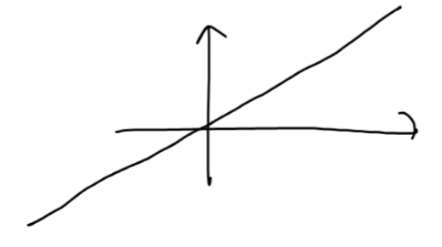
\includegraphics[width=0.3\linewidth]{nullmenge_gerade}
    \label{fig:nullmenge_gerade}
  \end{figure}
  \begin{equation*}
    N_Y(x)\definedas \Set{y\in \reals|(x,y)\in N}=\Set{\frac{x}{2}}
  \end{equation*}
  ist Nullmenge in \( \reals \).

\end{beispiel*}
\begin{proof}[Beweis von \ref{nullmenge_mal_punkt_ist_nullmenge}]
  Zu \( n\in \naturals \) wählen wir eine Überdeckung von \( N \) der Form \( \bigcup_{i\in \explain{\text{abzählbar}}{I_n}}Q_i^{(n)}\times P_i^{(n)} \) durch Quader \( Q_i^{(i)}\subset X \), \( P_i^{(i)}\subset Y \),
  \begin{equation*}
    \volume*{\bigcup_{i\in I_n Q_i^{(n)}\times P_i^{(n)}}}<2^{-n}\quad (\volume;=\mu\times \varv).
  \end{equation*}
  Dies liefert eine Überdeckung \( \bigcup_{k\in I}Q_k\times P_k \), \( I =  \) disjunkte Vereinigung aller \( I_n \) (wieder abzählbar) mit 
  \begin{equation*}
    \volume*{\bigcup_{k\in I}Q_k\times P_k}<\sum_{n\in \naturals} w^{-n}=\frac{1}{1-\frac{1}{2}}-1<\infty.
  \end{equation*}
  Jeder Punkt in \( N \) wird von dieser abzählbar unendlich oft überdeckt.

  Es gilt für \( R_k=Q_k\times P_k \)
  \begin{equation*}
    \volume{R_k}=\volume{Q_k}\cdot \volume{P_k}.
  \end{equation*}
  Also
  \begin{align*}
    \mu\times \varv(R_k)&=\Integrate{\characteristicfunction{R_k}{x,y}}{{(x,y)}}\\
    &=\Integrate{\p*{\Integrate{\characteristicfunction{R_k}{x,y}}{y,Y}}}{x,X}\\
    \implies \span \sum_{k=1}^{\infty}\Integrate{\p*{\Integrate{\characteristicfunction{R_k}{x,y}}{y,Y}}}{x,X}<\infty.
  \end{align*}
  Mit Beppo-Levi (\ref{beppo-levi-einfach}), angewendet auf
  \begin{equation*}
    f_n(x)=\sum_{k=1}^{n}\Integrate{\characteristicfunction{R_k}{x,y}}{y,Y},
  \end{equation*}
  folgt:
  \begin{equation}
    \sum_{k=1}^{\infty}\Integrate{\characteristicfunction{R_k}{x,y}}{y,Y} 
  \end{equation}
  konvergent für fast alle \( x \). Sei \( x_0\in X \) \sd \( \lim_{n \goesto \infty}f_n(x_0)<\infty \).

  Mit Beppo-Levi, angewendet auf
  \begin{equation*}
    g_n^{x_0}=\sum_{k=1}^{n}\characteristicfunction{R_k}{x_0,y}
  \end{equation*}
  folgt \( \sum_{k=1}^{\infty}\characteristicfunction{R_k}{x_0,y} \)
  konvergiert für fast alle \( y \).
  Sei \( y_0\in Y \), \sd  \( \lim_{n \goesto \infty}g_n^{x_0}(y_0)<\infty \) 
  \timplies \( (x_0,y_0)\not\in N \), 
  also \( y_0\not\in N_Y(x_0) \), 
  denn für \( (x_0,y_0)\in N \) ist \( \sum_{k=1}^{\infty}\characteristicfunction{R_k}{x_0,y_0}=\infty \).
\end{proof}
\begin{proof}[Beweis des Satzes von Fubini (\ref{fubini})]
  Zu zeigen ist:
  \begin{eigenschaftenenumerate}
    \item \label{fubini:funktion_in_stufenfunktionen_Y}\( f(x,\cdot)\in\stufenfunktionen(Y) \) für fast alle \( x\in Y \),
    \item \label{fubini:integral_in_stufenfunktionen_X}\( \Integrate{f(\cdot,y)}{y,Y}\in \stufenfunktionen[2](X) \),
    \item\label{fubini:funktion_integral_richtig} \( \Integrate{f(x,y)}{{(x,y)}}=\Integrate{\p{\Integrate{f(x,y)}{y,Y}}}{x,X} \).
  \end{eigenschaftenenumerate}
  Ist \( f=\characteristicfunction;{P\times  Q} \), \( P\subset X \), \( Q\subset Y \), so gelten \ref{fubini:funktion_in_stufenfunktionen_Y}, \ref{fubini:integral_in_stufenfunktionen_X}, \ref{fubini:funktion_integral_richtig} wegen \( \characteristicfunction{P\times Q}{x,y}=\characteristicfunction{p}{X}\characteristicfunction{Q}{y} \) \timplies \ref{fubini:funktion_in_stufenfunktionen_Y}, \ref{fubini:integral_in_stufenfunktionen_X}, \ref{fubini:funktion_integral_richtig} gelten für Stufen-Funktionen \( \stufenfunktionen[0](X\times Y) \)  (\ref{fubini:funktion_in_stufenfunktionen_Y}, \ref{fubini:integral_in_stufenfunktionen_X} mit \( \stufenfunktionen[0] \) statt \( \stufenfunktionen[2] \)) (weil diese Linearkombinationen von Funktionen der Form \( \characteristicfunction;{P\times Q} \) und das Integral linear).

  Sei nun \( f\in \stufenfunktionen[1](X\times Y) \). Wähle \( \p{\varphi_k}_k \subset \stufenfunktionen[0] \) und \( N\subset X\times Y \) Nullmenge \sd
  \begin{equation*}
    \varphi_k (x,y) \goesupto f(x,y) \quad \forall (x,y)\in (X\times Y)\setminus N\implies \Integrate{\varphi_k}{{(x,y)}}\goesupto \Integrate{f}{{(x,y)}}\tag{\( * \)}\label{eq:fubini:r0_zu_r1}
  \end{equation*}
  \thref{nullmenge_mal_punkt_ist_nullmenge} \timplies \( N_y(x_0)=\Set{y\in Y|(x_0,y)\in N} \) ist Nullmenge für fast alle \( x_0 \). Bezeichne \( \tilde{X}\subset X \) die Menge aller solchen \( x_0 \). Dann gilt für jedes fest gewählte \( x_0\in \tilde{X} \) \( \varphi_k(x_0,y)\goesupto f(_0,y) \) fast überall in \( Y \) und \( \p*{\varphi_k(x_0,\cdot)}\subset \stufenfunktionen[0](Y) \) und
  \begin{equation*}
    \Integrate{\varphi_k(x_0,y)}{y,Y}\goesupto \Integrate{f(x_0,y)}{y,Y}\quad \forall x_0\in \tilde{X}, \text{ also für fast alle } x\in X.
  \end{equation*}
  Es ist zudem
  \begin{equation*}
  \phi_k(x)\definedas \Integrate{\varphi_k(\cdot,y)}{y,Y}\in \stufenfunktionen[0](X)
  \end{equation*}
  und somit folgt:
  \begin{equation*}
    g\definedas\Integrate{f(\cdot,y)}{y,Y}\in \stufenfunktionen[1](X)
  \end{equation*}
  und
  \begin{equation}
    \Integrate{\varphi_k(x)}{x,X}\goesupto \Integrate{g(x)}{x,X},
  \end{equation}
  also
  \begin{equation*}
    \tag{\( ** \)}\label{eq:fubini:integral_integral_ueber_stufenfunktionen} \Integrate{\p*{\Integrate{\varphi_k(x,y)}{y,Y}}}{x,X}\goesupto \Integrate{\p*{\Integrate{f(x,y)}{y,Y}}}{x,X}
  \end{equation*}
  \timplies \ref{fubini:funktion_in_stufenfunktionen_Y} und \ref{fubini:integral_in_stufenfunktionen_X} (mit \( \stufenfunktionen[1] \) statt \( \stufenfunktionen[2] \)) für \( f\in \stufenfunktionen[1] \). \ref{fubini:funktion_integral_richtig} folgt ebenso: Es gilt \ref{fubini:funktion_integral_richtig} für \( \varphi_k\in \stufenfunktionen[0] \), also folgt die \Beh aus \eqref{eq:fubini:r0_zu_r1}, \eqref{eq:fubini:integral_integral_ueber_stufenfunktionen}. 

  Sei nun \( f\in \stufenfunktionen[2](X\times Y) \). Schreibe \( f=f_1-f_2 \), \( f_0\in \stufenfunktionen[1](X\times Y) \), \( f_j\in \stufenfunktionen[1](X\times Y) \). Dann gilt \ref{fubini:funktion_in_stufenfunktionen_Y} und \ref{fubini:integral_in_stufenfunktionen_X} (mit \( \stufenfunktionen[1] \) statt \( \stufenfunktionen[2] \)) für \( f_1 \) und \( f_2 \) separat und somit\ref{fubini:funktion_in_stufenfunktionen_Y} und \ref{fubini:integral_in_stufenfunktionen_X} für \( f \). Auch \ref{fubini:funktion_integral_richtig} gilt für \( f_1 \) und \( f_2 \) separat und da \( \Integrate{f_1(x,y)}{{(x,y)},X\times Y} \) oder \( \Integrate{f_2(x,y)}{{(x,y)},X\times Y} \) endlich ist, erfüllt auch \( f \) \ref{fubini:funktion_integral_richtig}.
\end{proof}
\timestamp{39:15}
\begin{beispiel}[und geometriche Interpretation des Integrals]
  \begin{equation*}
    \Integrate{2x+3y}{{(x,y)},\interval{a}{b}\times \interval{c}{d}}.
  \end{equation*}
  \( f(x,y)=2x+3y \) ist auf \( Q=\interval{a}{b}\times \interval{c}{d} \) stetig \timplies beschränkt \timplies \( f\in \lebesgueintegrablefunctions(Q) \) \timplies (mit Fubini)
  \begin{align*}
    \Integrate{(2x+3y)}{{(x,y)},Q}&=\Integrate{\p*{\Integrate{2x+3y}{y,\interval{1}{3}}}}{x,\interval{a}{b}}\\
    &=\Integrate{\p*{-\frac{1}{2}}(c-d)(3c+3d+4x)}{x,\interval{a}{b}}\\
    &=\frac{1}{2}(b-a)(d-c)(2(a+b)+3(c+d))\\
    &=\text{ Volumen unter der Fläche}
  \end{align*}
   \begin{figure}[H]
     \centering
     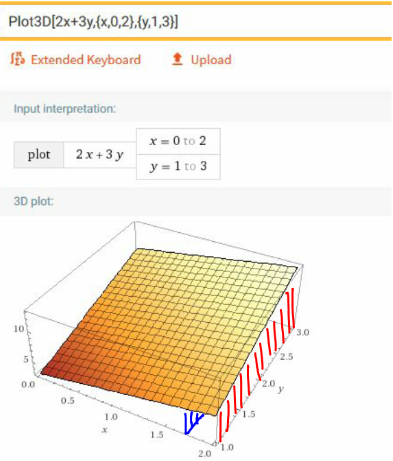
\includegraphics[width=0.5\linewidth]{volumen_unter_ebene}
     \label{fig:volumen_unter_ebene}
   \end{figure}
\end{beispiel}
\begin{beispiel*}
  \( \volume{\text{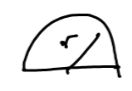
\includegraphics[height=\baselineskip]{flaeche_halbscheibe}}} \)
  \begin{figure}[H]
    \centering
    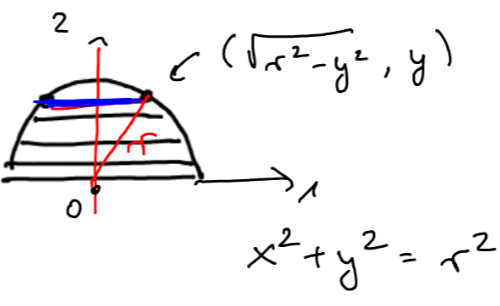
\includegraphics[width=0.4\linewidth]{halbscheibe_flaeche_erklaerung}
    \label{fig:halbscheibe_flaeche_erklaerung}
  \end{figure}  
  \begin{align*}
    \implies \volume{\text{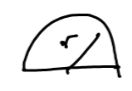
\includegraphics[height=\baselineskip]{flaeche_halbscheibe}}}&=\Integrate{1}{{(x,y)},\text{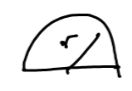
\includegraphics[height=0.3\baselineskip]{flaeche_halbscheibe}}}\\
    &=\Integrate{\p*{\Integrate{1}{x,\interval{-\sqrt{r^2-y^2}}{\sqrt{r^2-y^2}}}}}{y,\interval{0}{r}}\\
    &=\Integrate{2\sqrt{r^2-y^2}}{y,\interval{0}{r}}=\frac{1}{2}\pi r^2.
  \end{align*}
\end{beispiel*}
\begin{bemerkung}[Prinzip von Cavalieri]\label{prinzip_von_cavalieri}
  \begin{figure}[H]
    \centering
    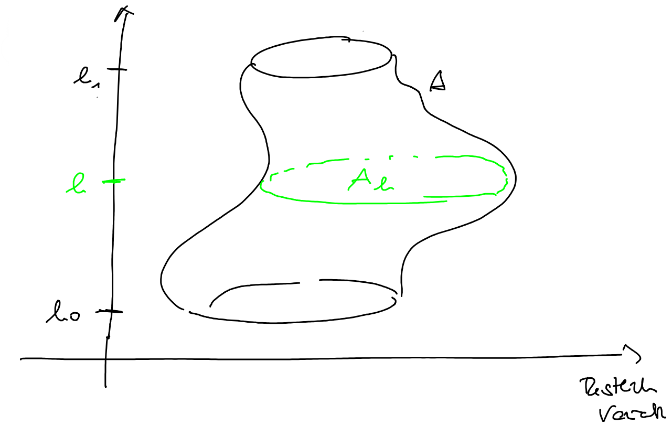
\includegraphics[width=0.5\linewidth]{prinzip_von_cavalieri}
    \label{fig:prinzip_von_cavalieri}
  \end{figure}
  \begin{equation*}
    \volume{A}=\Integrate{\volume{A_h}}{h,\interval{h_0}{h_1}}
  \end{equation*}
\end{bemerkung}
\begin{bemerkung}[Satz von Tonelli]
  \( f \) messbar, \( f\geq 0 \) \timplies \( f\in \stufenfunktionen[2] \) \timplies Fubini gilt.
\end{bemerkung}
